
\appendix

\section{Effect of Control Strength}

\begin{figure}[ht]
    \centering
    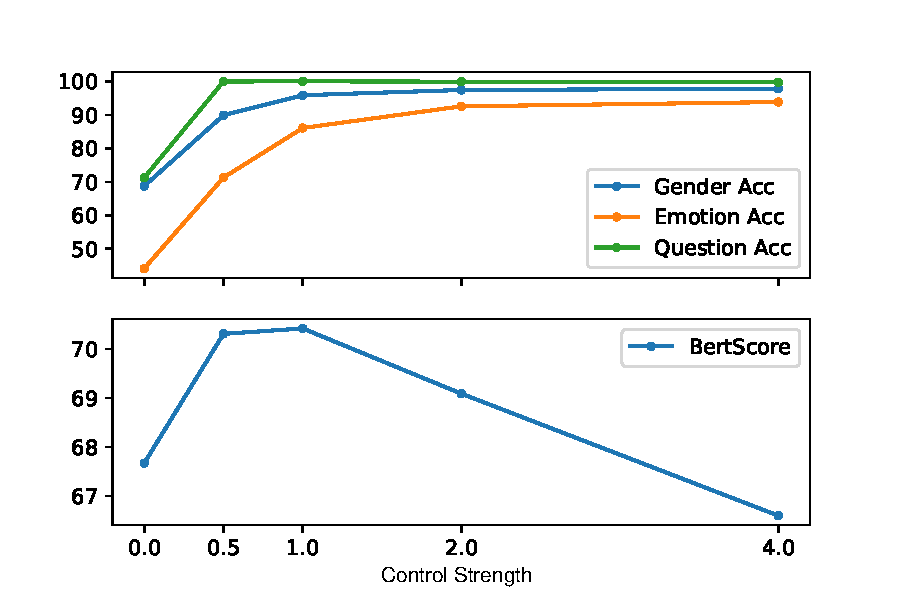
\includegraphics[width=1.0\columnwidth]{figures/parameter_tune.pdf}
    \caption{Effect of control strength on controllability and generation quality}
    \label{fig:parameter_tune}
\end{figure}

We show the effect of control strength $\alpha$ (\eqnref{eqn:dasc_logits}) on DASC's controllability and generation quality in Figure \ref{fig:parameter_tune}. From the trend shown in this figure, we can see that for \textit{Question} which is easy to control, we can already achieve perfect control with a low $\alpha$, while harder attributes like \textit{Emotion} would require a higher $\alpha$ to get a high success rate. Therefore, we may further hypothesize that a better balancing of the control accuracy of each attribute and the generation quality can be achieved by setting different control strengths for each aspect, like higher $\alpha$ for Emotion and lower $\alpha$ for Question. Careful tuning of the parameters or specific searching algorithms \citep{gu2022distributional} may serve the goal, and we leave this for future work.

\section{Experiment Details}

All experiments of the paper are conducted on a Linux server, and each experiment is run on a single NVIDIA A100 GPU. To avoid overfitting, we select the checkpoint with the best BertScore on dev set for final testing. We fix the random seed in experiment and report the results coming from a single run. Below we provide the specific details for the experiments on ESConv.

For experiments on ESConv \citep{liu2021towards}, we use the latest released version\footnote{\url{https://github.com/thu-coai/Emotional-Support-Conversation}}, which has 1,300 conversations, and we split them into 1,100/100/100 train/dev/test set, which contains 15,605/1,403/1,369 utterances each. In human evaluation, we further sample 15 utterances for each of the 7 emotional support strategies defined in the dataset (except the vague \textit{Other} class), and get 105 utterances in total. The meaning of \textbf{Sensibleness}$_{(1-4)}$ is similar to the experiment in the previous dataset: if the response is fluent, coherent with the context, and accords with commonsense. By \textbf{Usefulness}$_{(1-4)}$, we consider if the response dives deep in the problem faced by the support seeker, is comforting, contains useful suggestions or encourages in-depth further discussions. 

For all experiment methods, they use \texttt{bart-base}\footnote{\url{https://huggingface.co/facebook/bart-base}} as the base model, and are finetuned on the dataset for 6 epochs. The decoding method is top-$p$ sampling with $p=0.5$. DASC uses control weight $\alpha=1$ and classifier loss weight $\beta=0.1$, similar as the previous experiments.

\section{Examples and Visualizations}

In this section, we provide supplementary examples and figure visualizations. 

\begin{figure}[ht]
    \centering
    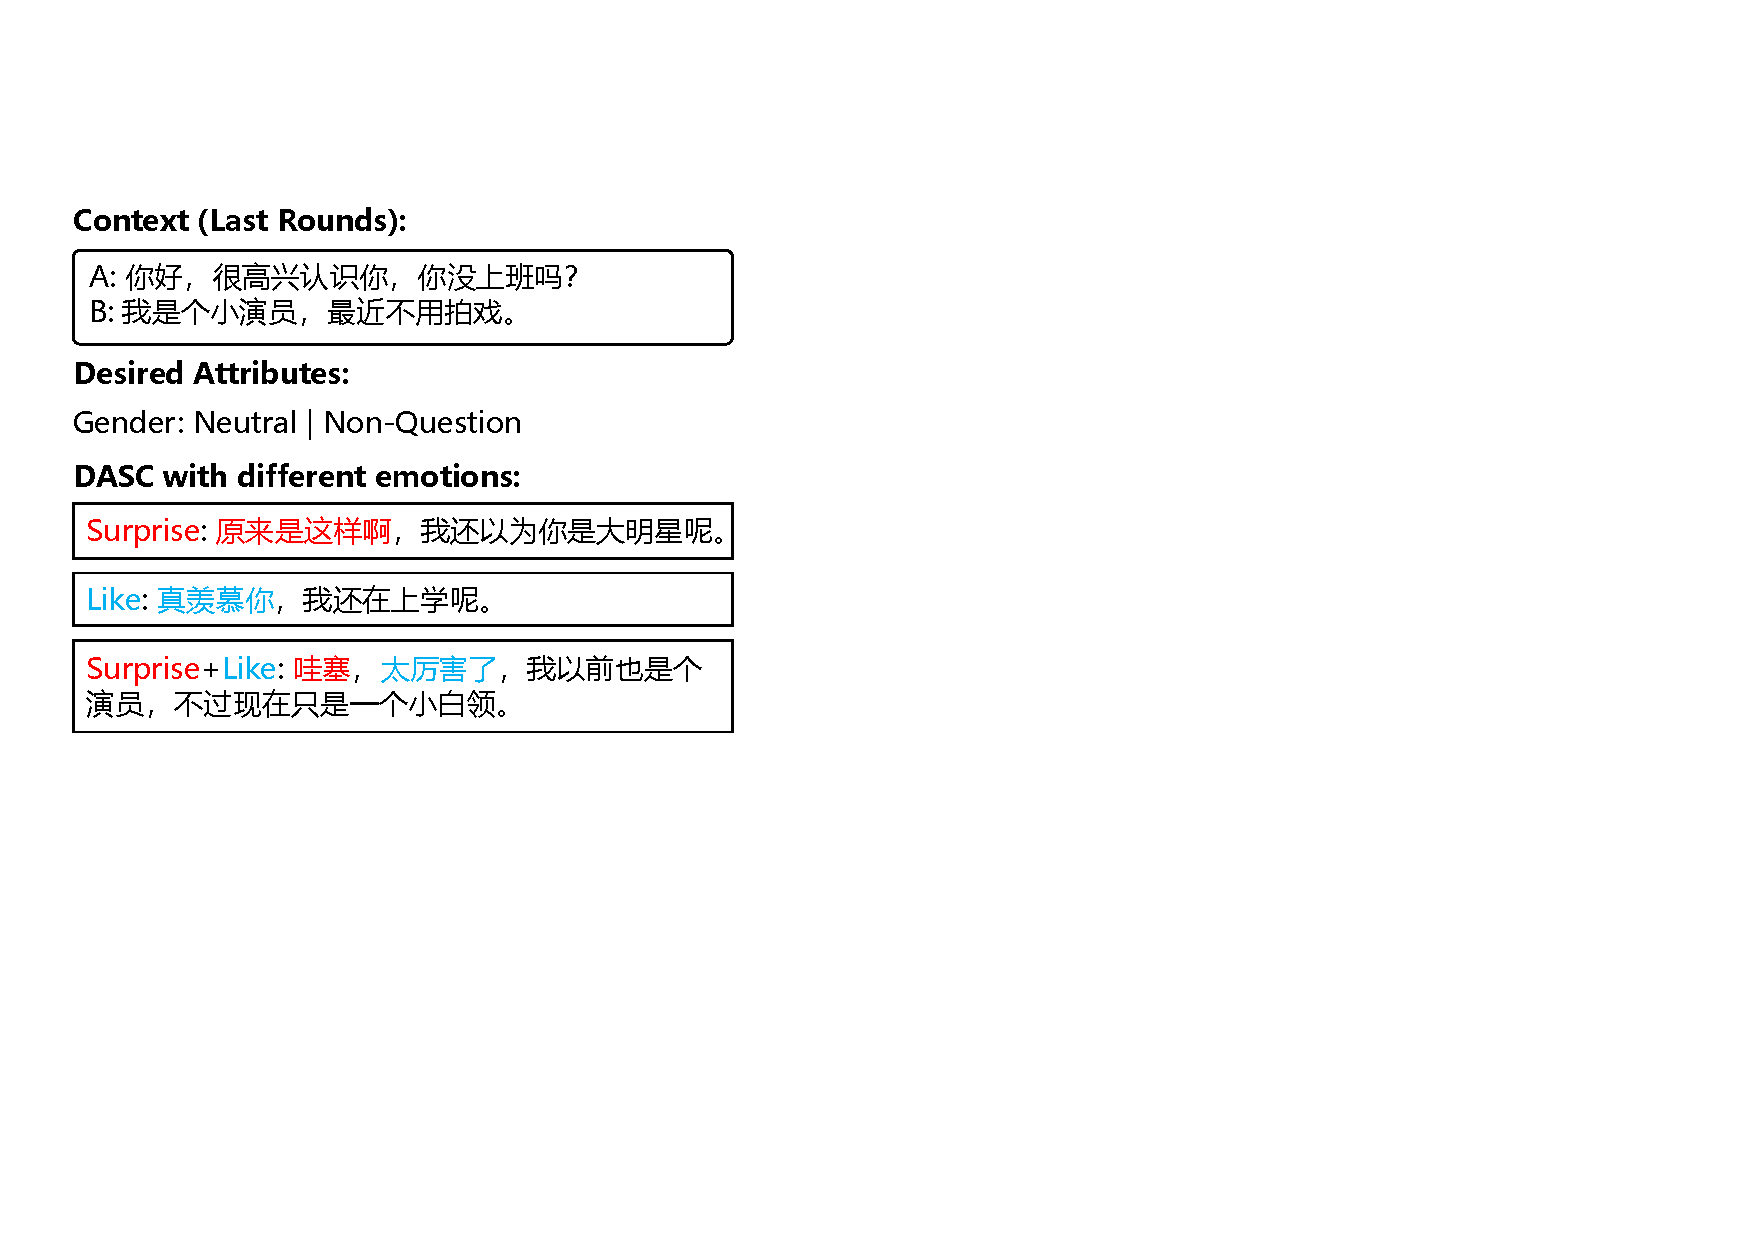
\includegraphics[width=1.0\columnwidth]{figures/compose_example1_zh.pdf}
    \caption{Original Chinese text for Figure \ref{fig:compose_example1_en}}
    \label{fig:compose_example1_zh}
\end{figure}

\begin{figure}[ht]
    \centering
    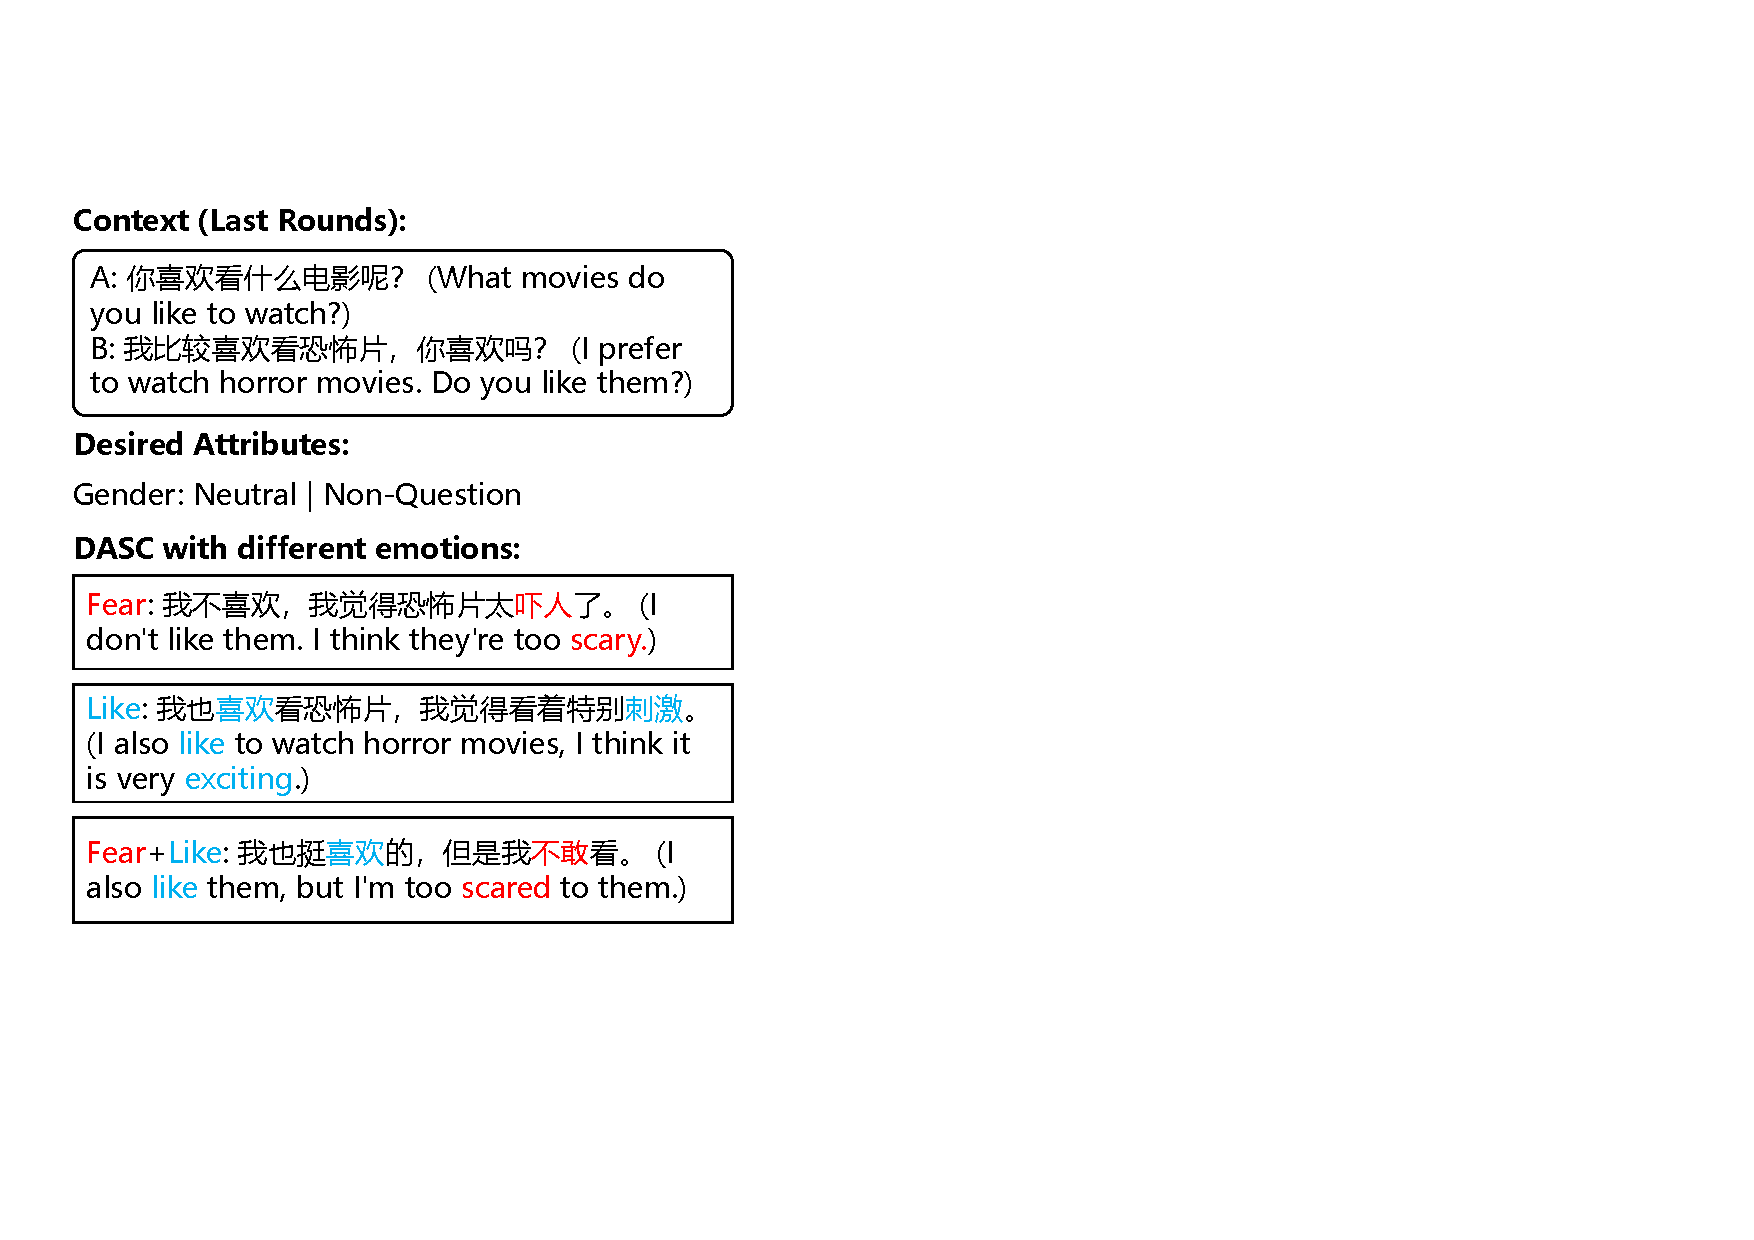
\includegraphics[width=1.0\columnwidth]{figures/compose_example2.pdf}
    \caption{Example of DASC composing \textit{Like} and \textit{Fear} emotion in the generated response.}
    \label{fig:compose_example2}
\end{figure}

Figure \ref{fig:compose_example1_zh} shows the original Chinese text for the emotion composition example in Figure \ref{fig:compose_example1_en}, and we provide another example in Figure \ref{fig:compose_example2}, which shows that DASC can even compose a positive emotion \textit{Like} and a negative emotion \textit{Fear} in the same response to express complex meanings. 

\begin{figure}[ht]
    \centering
    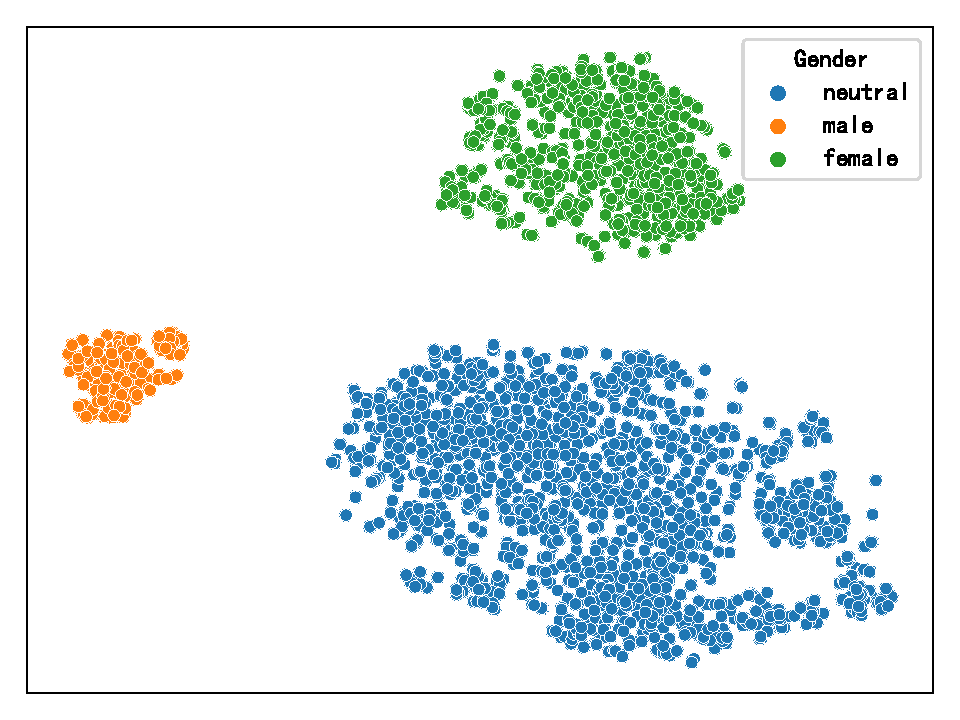
\includegraphics[width=1.0\columnwidth]{figures/gender_context_emb.pdf}
    \caption{Visualization of attribute context embedding of responses with different gender styles.}
    \label{fig:gender_context_emb}
\end{figure}

\begin{figure}[ht]
    \centering
    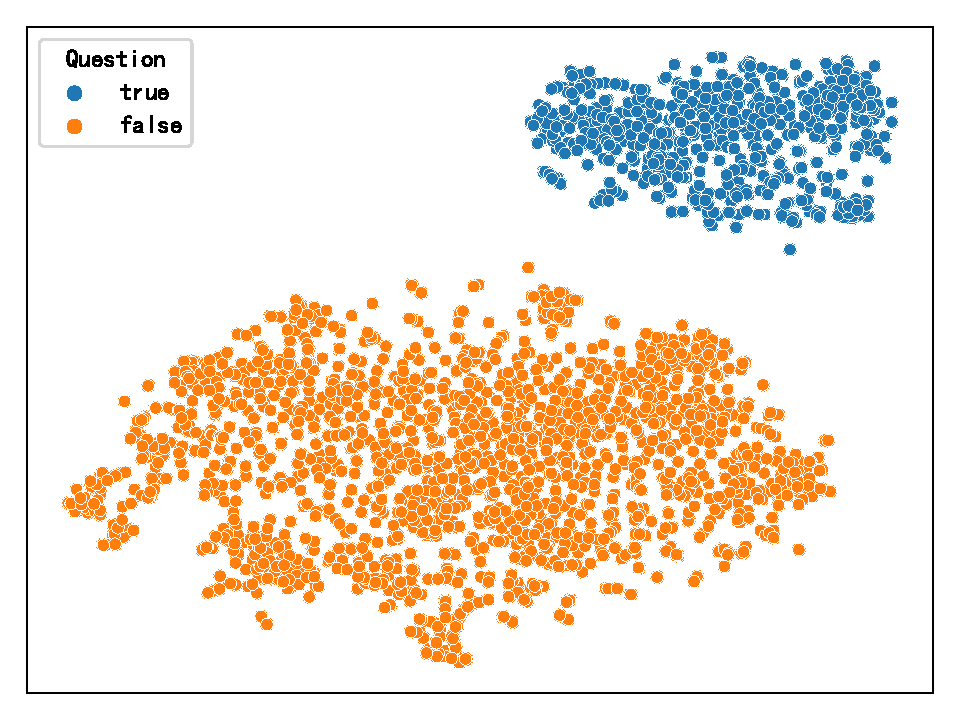
\includegraphics[width=1.0\columnwidth]{figures/question_context_emb.pdf}
    \caption{Visualization of attribute context embedding of responses with different question acts.}
    \label{fig:question_context_emb}
\end{figure}

We provide the t-SNE visualizations of attribute context embeddings of sentences with different \textit{Gender Style} and \textit{Question Act} in Figure \ref{fig:gender_context_emb} and Figure \ref{fig:question_context_emb}. We find similar results as we've seen for emotion, that the embeddings from different attributes are clearly separated.

\begin{figure}[htbp]
    \centering
    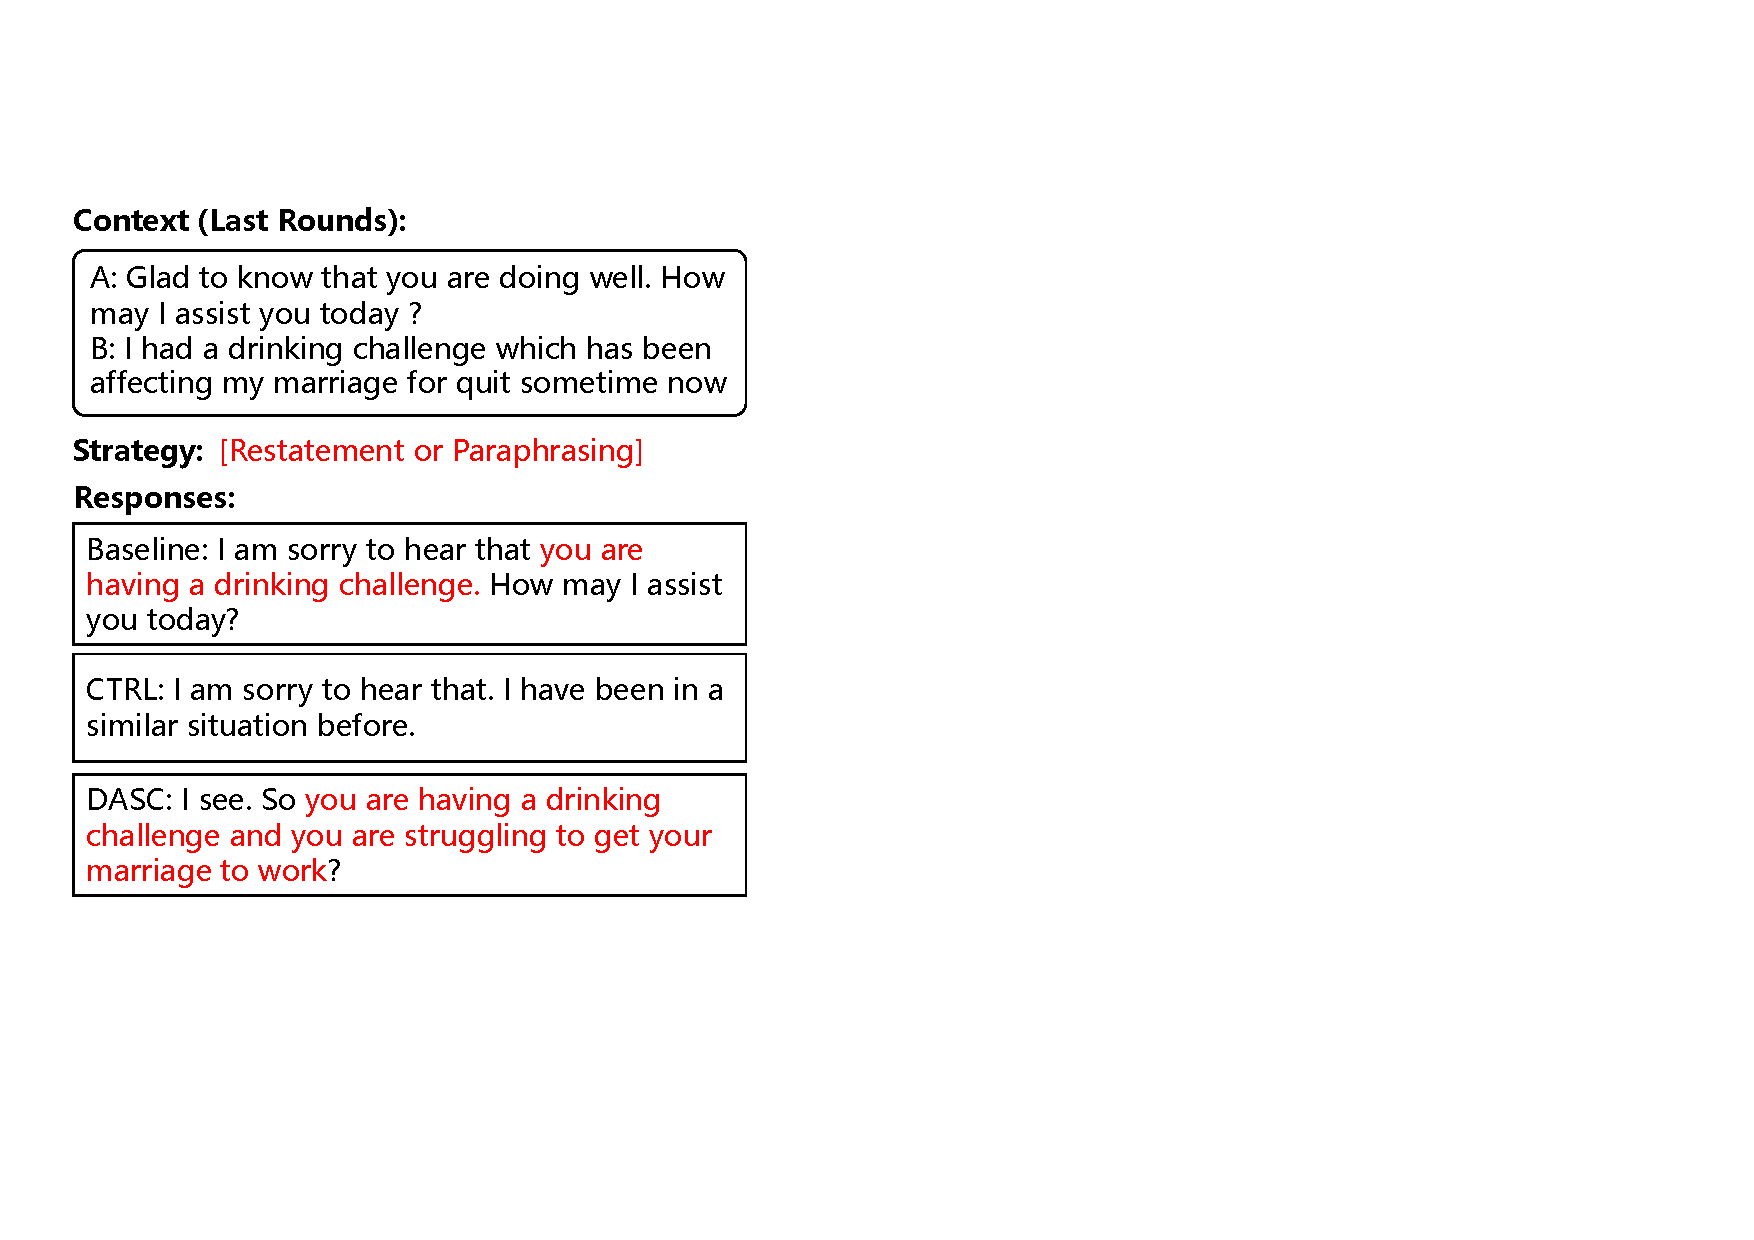
\includegraphics[width=1.0\columnwidth]{figures/esconv_example1.pdf}
    \caption{System generations in one example of ESConv, with the ``Restatement or Paraphrasing'' strategy.}
    \label{fig:esconv_example1}
\end{figure}

\begin{figure}[htbp]
    \centering
    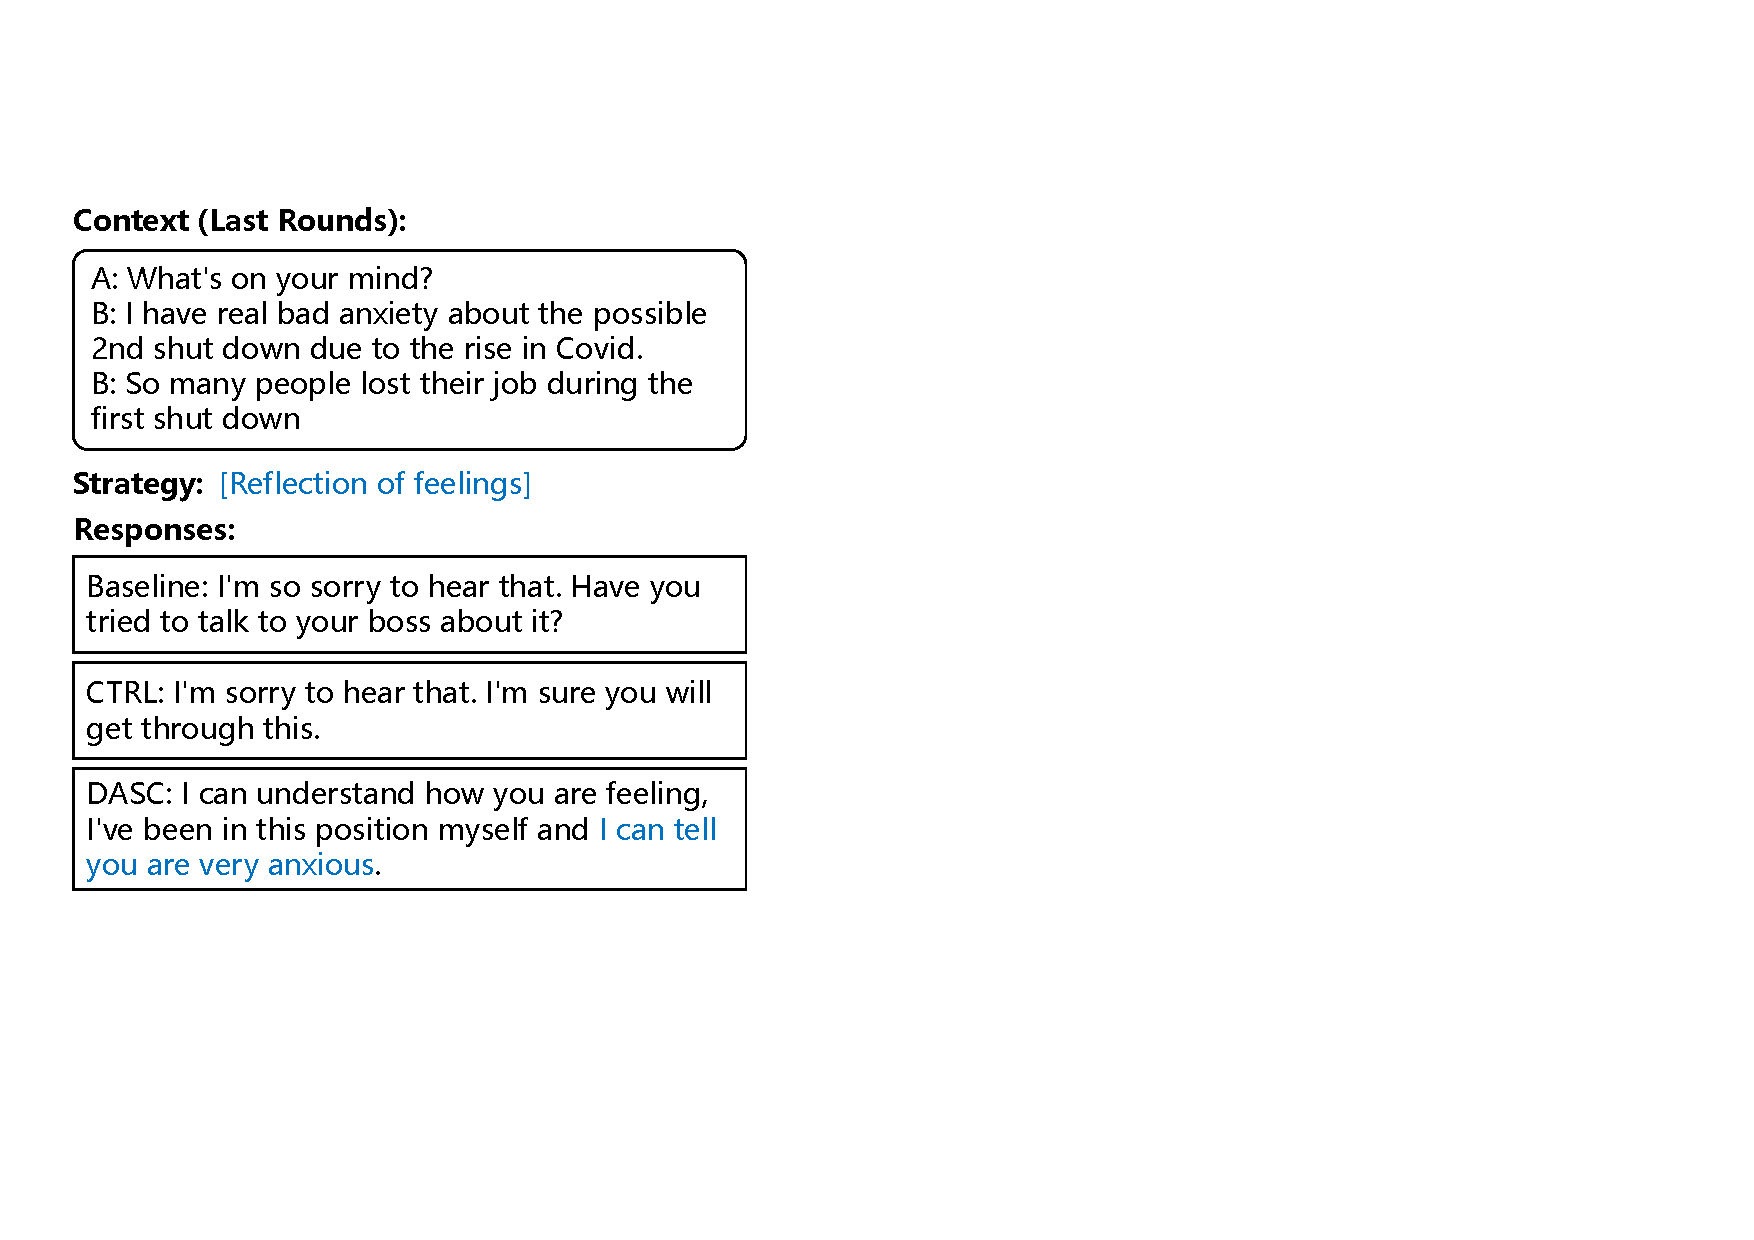
\includegraphics[width=1.0\columnwidth]{figures/esconv_example2.pdf}
    \caption{System generations in one example of ESConv, with the ``Reflection of feelings'' strategy.}
    \label{fig:esconv_example2}
\end{figure}

We also show 2 examples of the generated results on the ESConv. In Figure \ref{fig:esconv_example1}, both baseline and DASC successfully applied the desired strategy, while CTRL failed to do so. However, baseline also included a repetitive question at the end, while DASC gives a more comprehensive restatement, which exhibits a deep understanding of the situation and will be regarded as more helpful for the help seeker. In Figure \ref{fig:esconv_example2}, only DASC used the correct strategy in the generation, and such precise reflection of the anxious mood makes the response more sympathetic.